\begin{exercice*}
    La pyramide du Louvre est une pyramide régulière à base carrée de \Lg{35} de côté et de \Lg{22} de hauteur.

    \begin{enumerate}
        \item Faire un schéma.
        \item Calculer le volume $\mathcal{V}$ de cette pyramide.
        
        Donner la valeur exacte en \Vol[m]{} puis arrondie à l'unité.
        \item Sur une maquette, on construit une réduction de cette pyramide. Le côté de la base
        carrée de cette réduction mesure \Lg{7}.

        \medskip
        Calculer le coefficient de réduction.
        \item En déduire le volume $\mathcal{V}'$ de la pyramide sur la maquette.
        
        Donner la valeur exacte en \Vol{} puis arrondie à l'unité.
    \end{enumerate}

    \hrefMathalea{https://coopmaths.fr/mathalea.html?ex=3G22-1,n=3,i=1&v=l}
\end{exercice*}
\begin{corrige}
    %\setcounter{partie}{0} % Pour s'assurer que le compteur de \partie est à zéro dans les corrigés
    \phantom{rrr}

    \begin{multicols}2
    \begin{enumerate}                
        \item \phantom{rrr}
        
        \begin{tikzpicture}[scale=0.7]
            % \draw[help lines, color=black!30, dashed] (0,0) grid (12,8);                
            \coordinate (A) at (2,1);
            \coordinate (B) at (8,1);
            \coordinate (C) at (10,3);
            \coordinate (D) at (4,3);
            \coordinate (E) at (6,2);
            \coordinate (F) at (6,7);            
            
            \tkzDrawSegment(B,C);
            \tkzDrawSegment(F,C);
            \tkzDrawSegment(F,B);
            \tkzDrawSegment(F,A);
            \tkzDrawSegment[dashed](C,D);
            \tkzDrawSegment[dashed](D,A);
            \tkzDrawSegment[dashed](D,F);
            \tkzDrawSegment[dashed](D,B);
            \tkzDrawSegment[dashed](A,C);
            
            \begin{scope}[ dim style/.append style={red, dashed},
                dim fence style/.style={red, dashed}]                
                \tkzDrawSegment[dashed, dim={\(\Lg[m]{22}\),-3cm,right=2mm}](E,F)
                \tkzDrawSegment[dim={\(\Lg[m]{35}\),-5mm,below=2mm}](A,B)
            \end{scope}
            \tkzMarkRightAngle[fill=gray!20](F,E,B);
            \tkzMarkRightAngle[fill=gray!20](F,E,A);            
        \end{tikzpicture}
        \columnbreak        
        \item $\mathcal{V}_{\text{pyramide}} = \dfrac{1}{3}\times \mathcal{A}_{\text{base}}\times \text{hauteur}$.
        
        \medskip
        Donc $\mathcal{V} = \dfrac{1}{3}\times 35^2\times 22 = \dfrac{\num{26950}}{3} \Vol[m]{} \simeq\Vol[m]{8983}$.
        \medskip
        \item Soit $k$ le rapport de réduction, $k = \dfrac{7}{35}=\dfrac{1}{5}=\num{0.2}$.
        
        \medskip
        \item Si les longueurs sont multipliées par un rapport $k$, les volumes, qui sont homogènes à 
        des produits de trois longueurs sont donc multipliées par $k^3$.

        \medskip
        Donc $\mathcal{V}'=k^3\times \mathcal{V} = \num{0.2}^3\times\dfrac{\num{26950}}{3}=\dfrac{\num{1078}}{15}\simeq \Vol{72}$.
    \end{enumerate}
    \end{multicols}
\end{corrige}

